\documentclass[notes, xcolor=dvipsnames]{beamer}

\usetheme{Warsaw}

\usepackage{inputenc}
\usepackage{amsmath}
\usepackage{graphicx}

\title{Partially Redundant Fence Elimination for x86, ARM and Power Processors}
\subtitle{Robin M., Francesco Z.}

\author{Presented by \\ Akshay Gopalakrishnan}

\begin{document}

    \begin{frame}
        
        \maketitle

    \end{frame}


    \begin{frame}{Introduction}

        \begin{itemize}
            \item Usage of memory Fences/Barriers are expensive. 
            \item Compiling programs to hardware instructions want to avoid too many uses of fences.
            \item Fences can be redundant on compilation, thereby existing fence elimination optimizations.
            \item However, existing ones are either too constrained, or are not proven to be correct. 
        \end{itemize}
        
    \end{frame}

    \begin{frame}{Contributions}

        \begin{itemize}
            \item This paper proposes a more aggressive Fence optimization using Partial Redundancy Elimination technique used in Compiler Optimizations.
            \item The source language is C11, target hardware are x86, ARM and Power.
            \item Key idea is to represent fences and program instructions as a control flow graph with weighted edges.  
            \item This program graph is converted to a min cut problem, wherein the min-cut determines the location where fences are required.
            \item Using this information, other fences in the program can be removed.
        \end{itemize}
        
    \end{frame}


    \begin{frame}{Motivating Example}{Trivial}

        \begin{figure}
            \makebox[\textwidth][c]{
                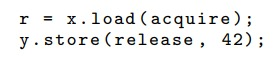
\includegraphics[scale=0.5]{Motiv_Ex_1_1.jpeg}
            }
            \caption{C program.}
        \end{figure}
        \begin{figure}
            \makebox[\textwidth][c]{
                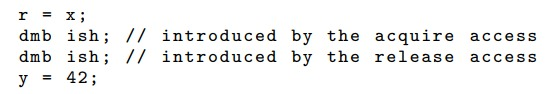
\includegraphics[scale=0.5]{Motiv_Ex_1_2.jpeg}
            }
            \caption{Mapping with ARM Fences.}
        \end{figure}
        
    \end{frame}

    \note{
        The example mapping here depicts the mapping of read/writes in C11 style to ARM equivalent memory access.
        In that sense, the semantics of a load-acquire requires adding fence after an ARM load. 
        Whereas the store-release requires adding fence before an ARM store.
        The fence used in essence ensures the semantics mentioned in \url{https://developer.arm.com/documentation/dui0489/c/arm-and-thumb-instructions/miscellaneous-instructions/dmb--dsb--and-isb}
        TLDR, \emph{dmb ish; dmb ish} is equivalent to having just one \emph{dmgb ish}.
    }

    \begin{frame}{Motivating Example: Slightly Complex}
        \begin{figure}
            \makebox[\textwidth][c]{
                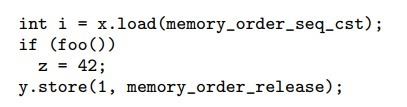
\includegraphics[scale=0.5]{Motiv_Ex_2_1.jpeg}
            }
            \caption{C program.}
        \end{figure}
        \begin{figure}
            \makebox[\textwidth][c]{
                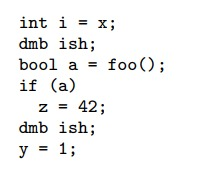
\includegraphics[scale=0.5]{Motiv_Ex_2_2.jpeg}
                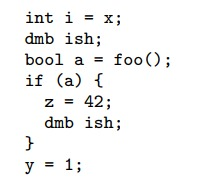
\includegraphics[scale=0.5]{Motiv_Ex_2_3.jpeg}
            }
            \caption{Two Possible Mappings with ARM Fences.}
        \end{figure}
        
    \end{frame}

    \note{
        In this example, depending on whether the conditional is satisfied, we can have either two consecutive \emph{dmb ish} (on true branch) or one \emph{dmb ish}, like the mapping on the right.
        But what we get is actually the mapping on the left, if we apply the mapping from memory accesses to ARM instructions naively.  
    }


    \begin{frame}{Motivating Example: Non-Trivial}
        
        \begin{figure}
            \makebox[\textwidth][c]{
                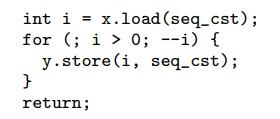
\includegraphics[scale=0.5]{Motiv_Ex_3_1.jpeg}
            }
            \caption{C program.}
        \end{figure}

    \end{frame}

    \note{
        Here is an example with sequentially consistent memory accesses.
        As per the ARM mapping, a sequentially consistent load must be mapped to a memory load followed by \emph{dmb ish}.
        Whereas for a sequentially consistent store, it is mapped to first a \emph{dmb ish} followed by the memory store, and finally again a \emph{dmb ish}.
    }

    \begin{frame}
        \begin{figure}
            \makebox[\textwidth][c]{
                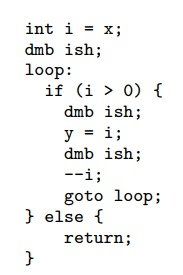
\includegraphics[scale=0.5]{Motiv_Ex_3_2_1.jpeg}
            }
            \caption{Naive Mapping}
        \end{figure}
        \begin{figure}
            \makebox[\textwidth][c]{
                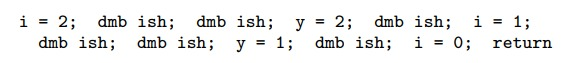
\includegraphics[scale=0.5]{Motiv_Ex_3_2_2.jpeg}
            }
            \caption{Instructions Executed for $x=2$}
        \end{figure}
        
    \end{frame}

    \note{
        Using the mapping rules, here is the ARM code.
        However, notice that for an example execution where $x=2$, we see the unnecessary fence consecutive pairs.
    }

    \begin{frame}
        \begin{figure}
            \makebox[\textwidth][c]{
                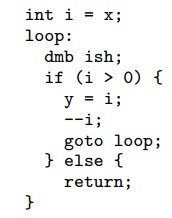
\includegraphics[scale=0.5]{Motiv_Ex_3_3_1.jpeg}
            }
            \caption{Optimal Mapping}
        \end{figure}
        \begin{figure}
            \makebox[\textwidth][c]{
                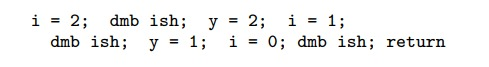
\includegraphics[scale=0.5]{Motiv_Ex_3_3_2.jpeg}
            }
            \caption{Instructions Executed for $x=2$}
        \end{figure}
        
    \end{frame}

    \note{
        What we want is a mapping like this. 
        The hint is that first, we need the read to $x$ be followed by a fence.
        This will happen in the first iteration of the loop body, before checking the loop condition. 
        After that, a write to $y$ is okay, as it is preceded by the fence already. 
        Since $i$ is thread-local, the fence placement w.r.t. $i$ is irrelevant.
        Again, in the next iteration, before we check the loop condition, \emph{dmb ish} is there, satisfying our requirement for mapping sequentially consistent load.
    }


    \begin{frame}{Key Idea}

        \begin{itemize}
            \item Represent fences as a relation between instructions.
            \item Correlate fence elimination via Partial Redundancy Elimination (PRE).
            \item Solve the PRE problem via min-cut problem, identifying minimal fence relations required.
            \item Remove the rest of the relations.   
        \end{itemize}
        
    \end{frame}

    \begin{frame}{First Step: Use Herding Cats Model}
        
        \begin{itemize}
            \item Represent program as a control flow graph.
            \item Nodes are all the memory accesses.
            \item Edges are control flow and fences.
            \item Fence edges are from prior memory access to later memory access.  
        \end{itemize}

    \end{frame}

    \begin{frame}{Second Step: Correlate with PRE}

        \begin{itemize}
            \item PRE problem identifies which computations are redundant.
            \item Treat fences as computations. 
            \item Treat the memory events after fence as a computation that requires the fence. 
            \item The PRE problem, then will identify the minimal fences required so that in every control flow to a given memory access, a fence is executed.
        \end{itemize}
        
    \end{frame}

    \begin{frame}{Third Step: PRE Solve as Min Cut}
        
        \begin{itemize}
            \item Connect the control flow graph to PRE via finding Min Cut. 
        \end{itemize}

        \begin{figure}
            \makebox[\textwidth][c]{
                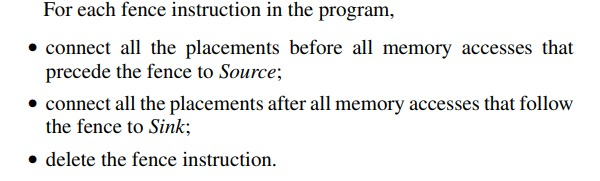
\includegraphics[scale=0.5]{Fence_Flow.jpeg}
            }
        \end{figure}
        
        \begin{itemize}
            \item The min cut is computed of the resulting graph. 
            \item Min cut indicates where the fences are required.
        \end{itemize}

    \end{frame}

\end{document}